\documentclass[a4paper,11pt]{article}
\usepackage[margin=2.5cm]{geometry}
\usepackage{parskip} % Package to tweak paragraph skipping

\usepackage{tikz} % Package for figure management
\usepackage{amsmath, amssymb}
\usepackage[amsmath, amsthm, thmmarks]{ntheorem}
\usepackage{hyperref}
\usepackage[utf8]{inputenc}
\usepackage[english]{babel}
\usepackage{dirtytalk} % quotation marks
\usepackage{csquotes}
\usepackage{caption} % multiline captions

\usepackage{biblatex} % bibliography
\addbibresource{bibliography.bib}

\theoremstyle{break}
\theoremindent=1cm
\theoremheaderfont{\kern-1cm\normalfont\bfseries}
\theorempreskip{0.4cm}
\theorempostskip{0.4cm}

\newtheorem{theorem}{Theorem}[section]
\newtheorem{definition}{Definition}[section]
\newtheorem{corollary}{Corollary}[theorem]
\newtheorem{lemma}[theorem]{Lemma}


\newcommand{\bib}{???}
\newcommand{\R}{\mathbb{R}}
\newcommand{\Nu}{\mathcal{N}}
\newcommand{\Ra}{\mathcal{R}}
\newcommand{\Exp}{\mathbb{E}}
\newcommand{\Mat}[2]{\mathbb{M}(#1, #2)}
\newcommand{\Part}[2]{\frac{\partial #1}{\partial #2}}

\DeclareMathOperator{\La}{\mathcal{L}}
\DeclareMathOperator{\diag}{diag}
\DeclareMathOperator{\bO}{\mathcal{O}}
\newcommand{\pll}{\parallel}

\title{Mathematics behind Machine Learning Algorithms}
\author{Hubert Bereś}
% \date{2018/01/08}

\begin{document}

\maketitle

\section{Introduction}

\subsection{Abstract}

Recently, both research and industry face many problems where the objective is to \say{guess} a function of multiple variables (features) based on its values at particular points (test samples). This essay focuses on two approaches, first linear multiple regression is discussed with rigorous algebraic background. It presents a proof of uniqueness of the optimal solution is proven and points towards ways of computing it through Moore-Penrose pseudoinverse.

In the second part limitations of such a model are illustrated and an alternative in the form of a neural network is presented. Difficulties in finding the optimal parameters are briefly discussed and a numerical solution together with a Back Propagation algorithm are derived.

\subsection{Machine learning context}

This essay focuses on functions from multiple real-valued inputs to a single real output
$$ f : \R^n \to \R $$
Such problem setting is very common and many other formats of input data like text, integer numbers or even images can be mapped onto $\R^n$ for the purposes of machine learning.

Treating each  component as a separate real-valued function the discussion below could be easily generalised to the case with multiple output variables.

The function $f$ is understood to approximate an unknown (complicated) process which we would like to model.
This essay focuses on {\tt parametrised}, {\tt supervised} machine learning.
Supervised means that we are given desired values of $f$ at certain points of its domain while parametrised means we assume $f$ can be determined by a vector of parameters $ \omega \in \Omega$ in some search space $\Omega$.
We write $ f(\omega; x) $ meaning that once parameters are set, $f$ can be evaluated at an arbitrary point $x \in \R^n$ of its domain.
The goal is then to decide on the right parametrisation and to compute optimal parameters $\omega$ within $\Omega$. We refer to this optimisation process as {\tt training} a model.

A good practical example of such modelling is to try to predict the price of a particular financial asset as a function of several other assets that may influence it with a complicated market mechanism. One can not describe this relation explicitly but we can hope to provide an approximation that follows general patterns of dependence between these prices.

In the context of machine learning we call the function $f$ a {\tt model} and we refer to the pairs of known input and output values as the {\tt training set}. It is often convenient to organise the training set into a matrix $H$ where each input value is represented by a row. Consequently we gather the corresponding values (also {\tt labels}) into a vertical vector $l$. The function $f$ acts on every row of a matrix separately, so that if the model was completely accurate we would get
    $$ f(H) = l $$

The usual way of measuring how well $f$ approximates the true process is by comparing $f(H)$ to the labels $l$ using sum of squared errors made on each sample. In matrix notation
$$ | f(\omega; H) - l |^2 $$
We refer to the above quantity as a {\tt training error} for parameters $\omega$.

Although initially only the training set is available to measure error, eventually $f$ should also approximate the process on data points that are similar to the ones in $H$ but not identical.

It comes out that due to random variation in the test sample, \say{simpler} models with slightly higher test error generalise better than the ones that tried to fit the noisy data more closely rather than following general patterns.
The issue of poor generalisation of too \say{complicated} models is known as {\tt overfitting}.

As a rule of thumb a model will overfit if it has more parameters \cite[pp112-113]{goodfellow}. Among models with the same parameter space the ones with smaller values of parameters (often measured by $ | \omega | $) tend to generalise better \cite[p119]{goodfellow}.
% this is a bold oversimplification but... I don't really want to go there as I'm short on space anyway.
With this motivation we first look into the simplest parametric model: linear regression.

\begin{figure}[b]
\centering
\captionsetup{width=0.8\linewidth}
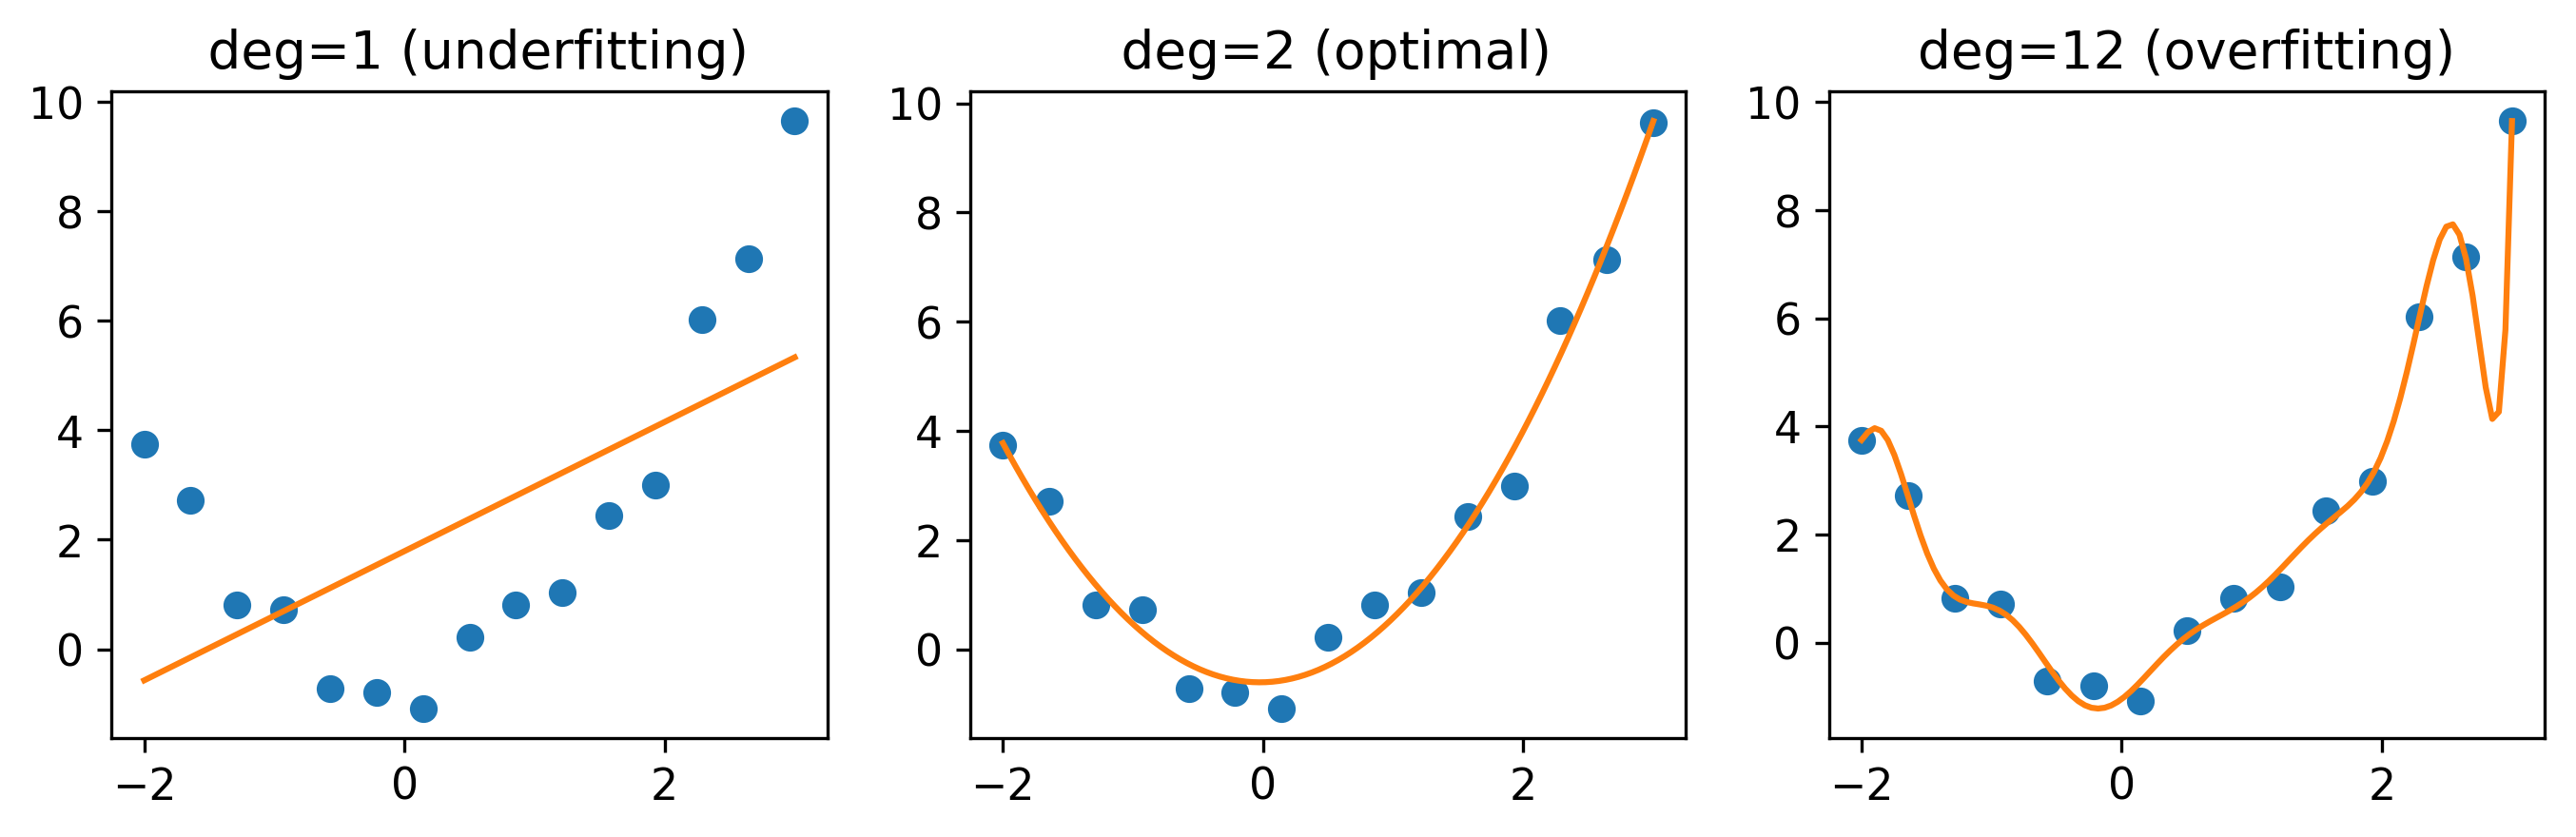
\includegraphics[width=0.8\linewidth]{polyfit.png}
\caption[]{
    \textit{Polynomial least-squares models with varying degree. \\
    Points generated by adding random noise to quadratic function;
    (left) insufficient number of parameters to follow the pattern;
    (centre) reasonable fit;
    (right) too many parameters follow noise.}
}
\end{figure} 

\begin{definition}[Multiple Regression]
    Given a real-valued $ m \times n$ matrix $H$ and a m-vector $l$ a Multiple Regression Model is a linear map $f \in \mathcal{L} ( \R ^n, \R)$ represented by a $ 1 \times n$ matrix $w$ such that
    \begin{equation}\label{def2}
        | H w - l | = \inf\limits_{x \in \R^n} | H x - l |
    \end{equation}
\end{definition}

In the following two sections we explore algebraic background that shows $ w $ can indeed be found and develop tools for computing it.

\pagebreak
\section{Multiple Regression}

\footnote{This section is a selection of statements from introduction in Albert's monograph on M-P pseudoinverse \cite[pp6-12]{albert}. Theorem proofs are adapted from there while Lemmas are my take on exercises.}
%
We start by stating several theorems closely related to the familiar notions of vector (sub)space, range and null-space.The first result provides a useful way of decomposing a vector into two components, with exactly one lying inside a vector subspace.Uniqueness of such decomposition will be useful when showing uniqueness of our optimal solution for the regression problem.

\subsection{Orthogonal decomposition}
Two vectors are perpendicular (denoted by $ a \perp b$) if and only if their scalar product is 0. Given a vector subspace $V \in \R^n$ we can think about vectors perpendicular to all its elements and denote them as $z \perp V$. We call a set of all such vectors the \texttt{orthogonal complement} of $V$:
$$ V^\perp := \{ v \in \R^n : v \perp V\} $$
Notice that $V^\perp \cap V = \{0\}$ and, since the scalar product is linear, that $V^\perp$ is itself a vector subspace. The following theorem provides a widely useful decomposition of an arbitrary vector:

\begin{theorem}[Orthogonal decomposition] \label{thm:projection}
    Let $z \in \R^n$ and $V \subset \R^n$ be a vector subspace. Then
    there exist unique $z_\perp \in V^\perp$ and $z_\pll \in V$ such that  
    \begin{equation}
        z = z_\perp + z_\pll
    \end{equation}
\end{theorem}

\begin{proof}
    The proof has been presented in the Geometry module.
\end{proof}

As we are interested only in finite-dimensional vector spaces the dimension formula
\begin{equation}\label{eq:dim_formula}
    dim(U + V) = dim(U) + dim(V) - dim( U \cap V)
\end{equation}
allows us to conclude an important property of the complement defined above:

\begin{lemma}\label{lem:double_perp}
    If $W$ is a finite-dimensional vector space and $V$ is its subspace then
    $$ V = (V^\perp)^\perp $$
\end{lemma}

\begin{proof}
    Pick an $x \in V$.
    By definition $ V^\perp = \{ y \in W : y \perp x \text{ for all } x \in V \}$ 
    hence for every $y \in V^\perp $ there is $x \perp y$.
    On the other hand 
    $ (V^\perp)^\perp = \{ x \in W : x \perp y \text{ for all } y \in V^\perp \}$ so 
    $x \in (V^\perp)^\perp$, i.e.
    $$ V \subset (V^\perp)^\perp$$

    Now as $W = V + V^\perp$ is finite-dimensional, let $dim(W) = n$ and $dim(V) = k$. 
    Knowing that $V \cap V^\perp = \{0\}$, by the dimension formula (\ref{eq:dim_formula}) we have
    $$ dim(V^\perp) = dim(W) - dim(V) = n - k $$
    We can apply the dimension formula again, noting that $ V^\perp \cap (V^\perp)^\perp = \{0\} $ to get:
    $$ dim((V^\perp)^\perp) = dim(W) - dim(V^\perp) = n - n + k = k $$

    We have shown $ V \subset (V^\perp)^\perp$ and $ dim(V) = dim((V^\perp)^\perp)$,
    hence $ V = (V^\perp)^\perp$.
\end{proof}

Once we have defined an orthogonal complement it is useful to relate them to the notions of null space and range.
The key result is a characterisation of a null space presented below.
Let $\Nu(H)$ resp. $\Ra(H)$ denote the null space resp. the range of a matrix $H$.

\begin{theorem} \label{thm:charact_nullspace}
    For any matrix $H \in \Mat{n}{m}$ the null space of $H$ is equal to the perpendicular complement of the range of $H^T$ in $\R^m$, i.e.
    $$\Nu(H) = \Ra^\perp(H^T) ~~\text{ where }~~ \Ra^\perp(H^T) := (\Ra(H^T))^\perp$$
\end{theorem}

\begin{proof}
    Pick any $x \in \Nu(H)$.
    We have $H x = 0$, implying $ y^T H x = 0$ for any $y \in \R^n$. Now
    \begin{equation}\label{eq:proof_nsp_char}
        y^T H x = (H^T y )^T x = 0
    \end{equation}
    which means that $x$ is orthogonal to all vectors of the form $ H^T y $, i.e. $ x \perp \Ra(H^T)$, showing $ \Nu(H) \subset \Ra^\perp(H^T)$. To see the other inclusion take $ y \in \Ra(H^T) $ and conclude from \eqref{eq:proof_nsp_char} that $ H x = 0$, i.e. $ x \in \Nu(H)$.
\end{proof}
Computing complements of both sides and applying Lemma \ref{lem:double_perp} gives an immediate corollary
    $$\Nu^\perp(H) = \Ra(H^T)$$

\subsection{Symmetric matrices}
We close this section with a few remarks on symmetric matrices and subspaces they generate. The importance of these results follows from the fact that symmetric matrices are always diagonalizable in $\R$ and hence play an important role in finding eigenvalues which come out to be closely related to our regression optimisation problem. 

\begin{lemma} \label{lem:charact_sym_nullspace}
    If $A$ is a symmetric matrix then $\Nu(A) = \Ra^\perp(A)$ and $\Nu^\perp(A) = \Ra(A)$.
\end{lemma}
\begin{proof}
    The claim follows immediately from Theorem \ref{thm:charact_nullspace} when we substitute $A^T = A$.
\end{proof}

\begin{lemma}
    \label{lem:nullspaces_hht}
    For an arbitrary matrix $H$,
    $$\Nu(H) = \Nu(H^T H) \text{ and } \Nu(H^T) = \Nu(H H^T)$$
\end{lemma}

\begin{proof}
    We will show mutual inclusion for the first equality. To prove that $\Nu(H) \subset \Nu(H^T H)$ pick $x$ such that $H x = 0$. Multiplying both sides by $H^T$ we get
    $$ H^T H x = H^T 0 = 0 $$
    implying $x \in \Nu(H^T H) $.
    To show the other inclusion, pick $x \neq 0$ such that $H^T H x = 0$. Multiplying from the right by $x^T$ yields
    $$ x^T H^T H x = (H x)^T H x = | H x |^2 = 0 $$
    implying $ H x =0 $ as required.
    
    The second equality of the lemma follows by a similar argument.
\end{proof}

The most interesting part of the above proof is completing a product of matrices to an expression of the form $v^T v = | v |^2 $ and using knowledge about norm of $v$ to reason about its structure.

An immediate corollary of Lemma \ref{lem:nullspaces_hht} provides analogous relationships between ranges:

\begin{corollary}\label{cor:equal_ranges}
    For an arbitrary matrix $H$
    $$\Ra(H) = \Ra(H H^T) \text{ and } \Ra(H^T) = \Ra(H^T H)$$
\end{corollary}

\begin{proof}
    We use the characterisation of null spaces \ref{thm:charact_nullspace} and compute orthogonal complements of each side. For example
    $$ \Nu(H) = \Ra^\perp (H^T) \text{ and } \Nu(H^T H) = \Ra^\perp ( H^T H )$$
    by Theorem \ref{thm:charact_nullspace}. From the last lemma we have
    $ \Nu(H) = \Nu(H^T H) $ so by the above:
    $$ \Ra^\perp (H^T) = \Ra^\perp ( H^T H ) $$
    or, by Lemma \ref{lem:double_perp}:
    $$ \Ra (H^T) = \Ra( H^T H ) $$
    as required. The other formula follows by a similar argument.
\end{proof}


\subsection{Moore-Penrose pseudoinverse}
\footnote{Content in this section is inspired on \cite[pp15-24]{albert}; significant changes were made in \ref{thm:regression_existence} and \ref{thm:regression_uniqueness}.}
Linear Algebra addresses a fundamental problem of solving a system of linear equations
$$ A x - b = 0$$
by introducing a notion of matrix inverse. If $x$ is a vector of unknown variables and certain conditions are met (including $A$ being a square matrix) one can obtain the solution $ x = A^{-1} b $.
As our problem of Multivariate Regression is almost identical in structure
$$ \inf | T x - l | $$
we would be interested in finding an analogous operation, say $ T \to T^+$ such that $ w = T^+ l$ gives the coefficients minimising the training error. 
Unfortunately we cannot use the matrix inverse since we expect $T$ to be rectangular (amount of test samples should be much bigger than number of parameters)!
On the other hand we do not hope to find an exact solution $ T w = l$, but rather just make the vectors $T w$ and $l$ ``as close as possible" under the standard norm.

This trade-off between precise solution which may not exist and an estimate with certain error that is always well defined motivates introduction of the Moore-Penrose pseudoinverse.

\subsection{Derivation}
First of all, we should make sure that the operator $T^+$ can be well defined, i.e. that given a multiple regression problem there exists a single vector of the \say{best} coefficients, minimising the training error.
The following two theorems assure existence of the solution and provide an interesting way of picking the best vector among those yielding the same error.

\begin{theorem}\label{thm:regression_existence}
With a matrix $H \in \Mat{m}{n}$ and $z \in \R^m$ the set
\begin{equation*}
    X := \{ x \in \R^n : | z - H x | = \inf\limits_{y \in \R^n} | z - H y | \}
\end{equation*}
        is not empty, i.e. there exists a vector $x$ minimising $| z - H x |$.
\end{theorem}
\begin{proof} % rework, using the shorter proof
    First write $z$ as $z = z_\pll + z_\perp$ with $z_\pll \in \Ra(H)$ and $z_\perp \in \Ra^\perp(H) = \Nu(H^T)$.
    By definition of range $H x \in \Ra(H)$ and so
    $$ z_\pll - H x \in \Ra(H) ~~ \implies ~~ z_\perp \perp z_\pll - H x $$
    meaning that $\langle z_\perp, z_\pll - H x \rangle$. Using that we obtain a lower bound:
    \begin{equation}\label{eq:upper_bound}
    | z - H x |^2 = | z_\perp + z_\pll - H x |^2 =
    | z_\perp |^2 + | z_\pll - H x |^2 + 2 \langle z_\perp, z_\pll - H x \rangle^2 = 
    | z_\perp | + | z_\pll - H x |^2 \geq | z_\perp |^2
    \end{equation}
    
    With equality if and only if $ z_\pll - H x $. Since $ z_\pll \in \Ra(H)$ such $x$ exists and so $X$ is not empty.
\end{proof}

\begin{theorem}\label{thm:regression_uniqueness}
    There is a unique vector $\hat{x}$ with minimum norm in X.
    Moreover, $\hat{x} \in \Ra(H^T)$.
\end{theorem}
\begin{proof}
    Pick $a, b \in X$ and use orthogonal decomposition:
    $$ a = a_\pll + a_\perp \text{ with } a_\pll \in \Nu(H),~~ a_\perp \in \Nu^\perp (H)$$
    $$ b = b_\pll + b_\perp \text{ with } b_\pll \in \Nu(H),~~ b_\perp \in \Nu^\perp (H)$$
    Notice that by definition of $a$ and $b$ we have
    $$ H a - H b = z_\pll - z_\pll = 0 ~~ \implies a - b \in \Nu(H)$$
    while on the other hand this difference can be written as
    $$ a - b = (a_\pll - b_\pll) + (a_\perp - b_\perp) \in \Nu(H)$$
    which implies $ a_\perp - b_\perp \in \Nu(H) $. Yet from the fact that $\Nu^\perp (H)$ is a vector space we have $ a_\perp - b_\perp \in \Nu^\perp (H)$. The only vector in $ \Nu^\perp (H) \cap \Nu (H)$ is $0$ proving $ a_\perp = b_\perp$.
    
    We have shown that any two solutions in $X$ share the same projection onto  $\Nu^\perp (H) = \Ra(H^T)$, meaning $a_\perp$ is determined by $z$.
    The only difference is the component lying in $\Nu(H)$. Clearly
    $$ | a |^2 = | a_\perp |^2 + |a_\pll |^2 \geq |a_\perp |^2$$
    so norm of $a$ is minimal if and only if $a_\pll = 0$, hence only one vector $a_\perp = \hat{x} \in X$ minimises the norm.
    By corollary of \ref{thm:charact_nullspace} we obtain $ \hat{x} \in \Nu^\perp (H) = \Ra(H^T) $ as required.
\end{proof}
Now as we have shown the solution exists and is unique if we settle for minimal norm as our secondary criterion of choice, we can construct an explicit formula for $a$ in terms of $z$ and $H$.

% there is a theorem 3.2 (normal equations) proven here in the book yet the derivation of MP doesn't seem to depend on it.
% Basically it says that  a can be obtained by picking y s.t. H^T H H^T y = H^T z and then a = H^T y.

The following two lemmas will guarantee that the limit involved in this definition exists:

\begin{lemma}\label{lem:invertible_1}
    For any nonzero $\delta$ the matrix $H^T H + \delta^2  I_m$ is invertible.
    \label{thm:invertible}
\end{lemma}
\begin{proof}
    Reasoning by contradiction suppose that for some $x \in \R^n \setminus \{0\}$ we have
    $$ (H^T H + \delta^2  I_m) x = 0 $$ % vector
Multiplying both sides by $x^T$ we obtain
    $$ x^T (H^T H + \delta^2  I_m) x = 0 $$ % scalar
    $$ x^T H^T H x + \delta^2 x^T x = 0 $$
    $$ | H x |^2 + \delta^2 | x |^2 = 0 $$
This is a contradiction as $ x \neq 0 \implies | x | > 0 $ and $ \delta^2 > 0$ by assumption.
Hence $\Nu(H^T H + \delta^2  I_m) = \{0\} $ and so the matrix is invertible.
\end{proof}

\begin{lemma}\label{lem:limit_existence_1}
    For a real symmetric matrix A, the following two limits exist and are equal:
    \begin{equation}
        H^+ := \lim_{\delta \to 0} A ( A + \delta I) ^{-1}
            = \lim_{\delta \to 0} ( A + \delta I) ^{-1} A
    \end{equation}
\end{lemma}

\begin{proof}
    Since $A$ is symmetric it has real eigenvalues and is diagonalizable.
    Let $T$ be orthogonal and $D := \diag (\lambda_1, \lambda_2, \ldots, \lambda_n)$ such that
    \begin{equation}
    \label{eq:aDiag}
        A = T D T^T = T D T^{-1}
    \end{equation}
    
    Let $ \delta_0 := min\{ | \lambda_i | : i \in {1, 2, \ldots, n}, \lambda_i \neq 0 \}$ and restrict
    $ \delta$ so that $ 0 <  | \delta | < \delta_0$.
    
    Now $(A + \delta I)$ is non-singular since for $ | x | = 1$ we have $ | A x | \geq \delta_0 > \delta$
    implying $ | (A + \delta I) x | > 0 $.
    As inverse is well-defined, for any $z = z_\perp + z_\pll$ decomposed with respect to range of $A$ we have
    $$ A z = A z_\pll$$
    On the other hand $z_\pll \in \Ra(A)$ so we can find $x_0$ such that $ z_\pll = A x_0$. Now
    $$ (A + \delta I)^{-1} A z = (A + \delta I)^{-1} A (A x_0) $$
    Which using \eqref{eq:aDiag} can be written as
    $$ (A + \delta I)^{-1} A z =
    (T(D + \delta I) T^{-1})^{-1} t D^2 T^{-1} x_0 =
    T (D + \delta I) D^2 T^{-1} x_0
    $$
    By considering each component of the diagonal separately, it is easy to see that
    $$ \lim_{\delta \to 0} (D + \delta I)^{-1} D^2 = D $$
    And hence, substituting back to the original limit we obtain
    $$ \lim_{\delta \to 0} ( A + \delta I) ^{-1} A z = T D T^T x_0 = A x_0 = z_\pll $$
    An analogous argument works for the other limit.
\end{proof}

Notice that it came out that $ H^+ z = z_\pll$ meaning that multiplication by $H^+$ projects $z$ onto $\Ra(A)$. Now we are finally in position to define Moore-Penrose pseudoinverse:

\begin{definition}[Moore-Penrose pseudoinverse]
    Let $H \in \Mat{m}{n}$.
    The Moore-Penrose pseudoinverse of $H$ is defined as
    $$ H^+ = \lim_{\delta \to 0} ( H^T H + \delta^2 I) ^{-1} H^T $$
\end{definition}

Note that if $H$ is invertible, this definition yields $H^+ = H^{-1}$. This is an expected property since if $H$ is invertible, there exists an exact solution to $ H x = z $ computed as $ H^{-1} z$.

We have seen in Lemma \ref{lem:charact_sym_nullspace} that $H^T H$ is symmetric which means $H^+$ is well defined by Lemma \ref{lem:limit_existence_1}. The following theorem shows that $ H^+$ indeed provides a minimum norm regression solution.

\begin{theorem}\label{thm:mp_solves_regression}
    For any $H$ and $z$ of appropriate dimensions, the vector $a = H^+ z$ is the one of minimal norm minimising $ | z - H x | $.
\end{theorem}

\begin{proof}
    Again, decompose $z$ into projections $z_\pll \in \Ra(H)$ and $z_\perp \in \Ra(H)^\perp = \Nu(H^T)$ and let $x_0$ belong to the preimage of $z_\pll$ i.e. $H x_0 = z_\pll$. Notice that
        $$ H^T z = H^T z_\pll = H^T H x_0$$
    so the Moore-Penrose pseudoinverse of $z$ can now be written as:
        $$ a = H^+ z
         = \lim_{\delta \to 0} (H^T H + \delta^2 I)^{-1} H^T H x_0
        $$
    As noted after the proof of Lemma \ref{lem:limit_existence_1}, $a$ is a projection of $x_0$ onto the range of $ A = H^T H $, while by Corollary \ref{cor:equal_ranges} we have $\Ra(H^T) = \Ra(H^T H)$.
    Hence $a$ is a projection of $x_0$ onto $\Ra(H^T)$ which, as in Theorem \ref{thm:regression_uniqueness} is the unique minimal norm solution for multiple regression.
\end{proof}

\subsection{Properties and applications}

Here we present without proof several results about the properties of the pseudoinverse itself and its applications. The following corollary is very useful as it expresses various projections discussed in the previous sections in terms of the pseudoinverse; once $ H^+ $ is known, the projections can be computed just by matrix multiplication. The proof is based on Theorem \ref{thm:mp_solves_regression} combined with various characterisations of ranges and null-spaces we have derived above.

\begin{lemma}
    For any vectors $z$ and $x$
    \begin{enumerate}
        \item $ H H^+ z $ is the projection of $z$ on $\Ra(H)$
        \item $ (I - H H^+) z $ is the projection of $z$ on $\Nu(H^T)$
        \item $ H^+ H x$ is the projection of $x$ on $ \Ra(H^T)$
        \item $ (I - H H^+) $ is the projection of $x$ on $ \Nu(H)$
    \end{enumerate}
\end{lemma}

To better understand the structure of the pseudoinverse, it is helpful to consider special cases.
\begin{lemma}[Scalar matrix]
    For a 1 by 1 matrix H the pseudoinverse is given by:
    $$ H^+ = \begin{cases}
        0~~~           \text{ if } H = 0\\
        \frac{1}{H}~~ \text{ if } H \neq 0
    \end{cases}$$
\end{lemma}
\begin{lemma}[Diagonal matrix]
    If $D = diag(d_1, d_2, ..., d_n)$ is a diagonal matrix then
    $$ D^+ = diag(d_1^+, d_2^+, ..., d_n^+) $$
\end{lemma}
\begin{lemma}[Symmetric matrix]
    If $A$ is a symmetric matrix diagonalized as $A = T D T^T $ then
    $$ A^+ = T D^+ T^T$$
\end{lemma}

Observing behaviour of the pseudoinverse for eigenvalues close to zero we see a discontinuity: small but non-zero value results in a large inverse while zero is mapped to zero. For example
$$ A = \left( \begin{matrix}
1 & 0 \\
0 & 0 \\
0 & 0
\end{matrix} \right) ~~~~
B = \left( \begin{matrix}
1 & 0 \\
0 & 0 \\
0 & 0.001
\end{matrix} \right)$$
are \say{almost identical} matrices, yet have drastically different pseudoinverses
$$ A^+ = \left( \begin{matrix}
1 & 0 & 0\\
0 & 0 & 0
\end{matrix} \right) ~~~~
B^+ = \left( \begin{matrix}
1 & 0 & 0\\
0 & 0 & 1000
\end{matrix} \right)$$

This phenomenon makes it challenging to compute pseudoinverse directly from the definition in a numerically stable way. Luckily, an alternative formula can be derived which is based on the singular value decomposition (SVD). This method is nowadays the most popular in computer libraries. Detailed discussion is out of scope of this essay, yet we state the result.
\begin{lemma}[Pseudoinverse from SVD]
    For a positive semidefinite normal matrix $H$ with singular value decomposition $H = U \Sigma V^*$ where $U$ and $V$ are unitary matrices and $\Sigma$ is a rectangular diagonal matrix with non-negative entries, the pseudoinverse can be written as:
    $$ H^+ = V \Sigma^+ U^* $$
\end{lemma}

\section{Neural networks}

\footnote{This section is my summary of Highams' article \cite{higham} and an extensive book by Goodfellow et all. \cite{goodfellow} in comparison with regression models. Statements and proofs on Back Propagation are taken from \cite{higham}.}
%
The second part of this essay is dedicated to an alternative, non-linear method of modelling $ f : \R^n \to \R$. A more complicated model implies we use more parameters to describe it, in turn making the optimisation problem significantly harder to solve. Only modern advances in computer algebra made such approach feasible in real-life scenarios.

A widely used model for $f$ is so-called Neural Network. It is worth noting that despite a very suggestive name this model is only loosely inspired by biological structure of our brains and does not aspire to reproduce our way of solving problems. This essay treats Neural Networks purely as a way of composing functions, ignoring the \say{historical} background.

\subsection{Non-linear structure}
To get a general idea about the techniques used to construct an optimal search space, let us analyse several shortcomings of a linear model and propose some modifications.

A linear function is unable to model situations when the outcome depends 'discretely' on one of the input parameters.
For example the step function with threshold $c \in \R$ defined as
$$ f(x) =
\begin{cases}
    0,& \text{if } x\leq c\\
    1,& \text{if } x > c
\end{cases}$$
can not be well approximated by $L(x) = a x  + b$.

\begin{figure}[tph]
    \centering
    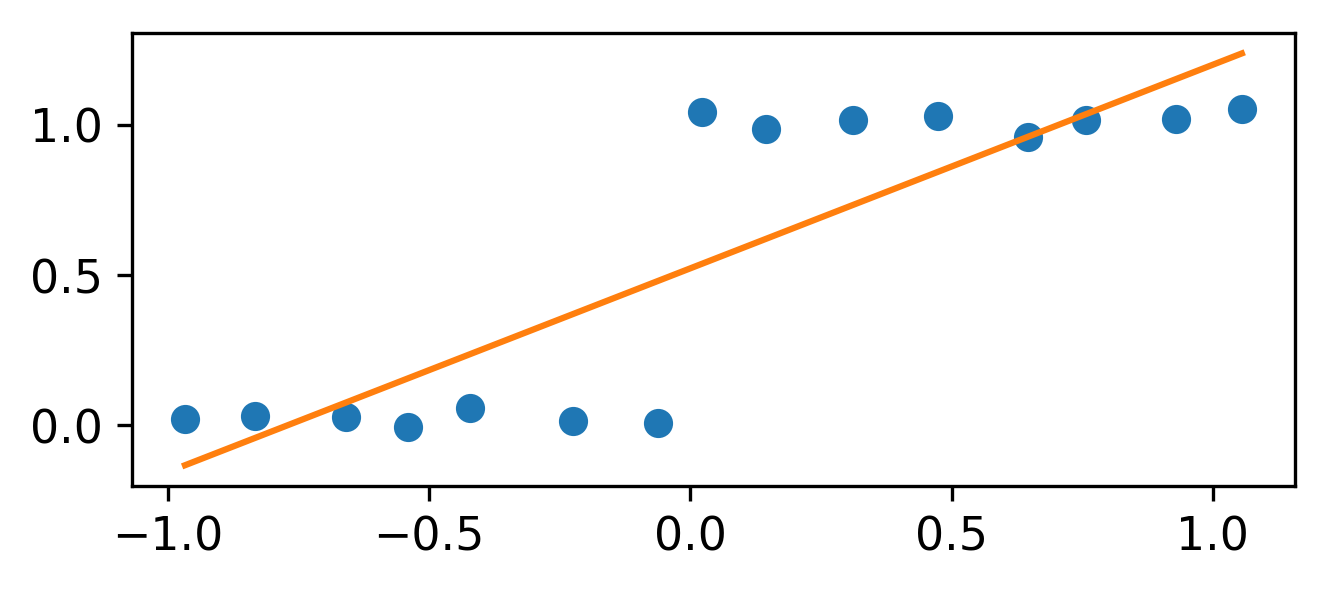
\includegraphics[width=0.4\linewidth]{step_linfit.png}
    \caption{\textit{Attempt to fit a linear model to samples from (noisy) step function with threshold 0.}}
\end{figure}

In order to model such behaviour, we will introduce to our model so-called activation function - a non-linear component  that imitates the step function. As optimisation procedures often rely on differentiation with respect to $x$, a common choice of activation function is the following:

\begin{definition}[Sigmoid function]
    $$ \sigma(x) = \frac{1}{1 + e^{-x}}$$
\end{definition}

In practice $f$ often depends on a non-additive combination of input variables, for example on a product $(x_1, x_2) \mapsto x_1 x_2$.
Again, modelling with a linear function gives a poor approximation here.
There are many ways of addressing this issue, which can be described in abstract terms as finding a preprocessing function $ \theta : \R^n \to \R^m$ that maps the original input to a space of features linearly influencing $f$. The model becomes $ f = f_1 \circ \theta $.

There is a variety of methods for finding $\theta$, often involving human expertise and trial and error.
Neural Networks attempt to automate this process by composing linear models denoted by $L$ with $\sigma$ i.e. the sigmoid function applied component-wise.
The complete model then looks like:
$$ f = (\sigma \circ L_{\La}) \circ (\sigma \circ L_{\La - 1}) \circ \ldots \circ (\sigma \circ L_{1}) $$
where
$$ L_i : \R^{n_{i-1}} \to \R^{n_{i}} \text{ for } i \in \{1, 2, \ldots, \La \} $$
$$ L_i(x) = W_i x + b_i $$
% !!! there should be one less matrices than the levels!
with $ n_0 $ denoting dimension of the input vector and the remaining $ n_i $ dimensions of the intermediate spaces, chosen arbitrarily. For convenience, just as in the linear case, set $ n_{\La} = 1 $. The components $ (\sigma \circ L_{i}) $ are called layers of the network.

\subsection{Training}

Assuming we have specified the number of layers and their dimensions, model $f$ is parameterised by values of $ b_1, b_2, \ldots, b_{\La} $ and $ W_1, W_2, \ldots, W_{\La} $, jointly denoted as $ \omega \in \Omega $.
As in the regression, given $H$ and $l$ representing the training set and labels we look for $ \omega $ minimising
    $$ C(\omega) =  \frac{1}{N} | f(\omega; H) - l |^2  $$
Contrary to the linear model case, we have no guarantee that this expression is a convex function of $ \omega $ and there is no known algebraic method of finding optimal parameters.

\subsection{Gradient Descent}
Since $C$ is a differentiable function, one can find its (local) minimum by iteratively moving in the direction of the steepest descent, i.e. in the direction of negative gradient
$ - \nabla C  = - ( \frac{\partial C}{\partial \omega_1}, \frac{\partial C}{\partial \omega_2, }, ..., \frac{\partial C}{\partial \omega_n})$.
Given an initial guess $\omega_0 \in \Omega$ such algorithm computes
    $$ \omega_{n+1} = \omega_{n} - \nabla C (\omega_n) h $$
where $h > 0$ is so-called step size. This optimisation algorithm is known as Gradient Descent.

Even assuming that the method converges (it can be made quite robust by tuning step size), there are two fundamental problems.
First, there is no guarantee of finding a global minimum.
As a dimension of the search space $ \Omega $ grows, finding an initial guess that leads to the optimal solution gets harder.
Yet this is not as detrimental since even a local minimum can provide a good accuracy.

The second problem is that computation of $\nabla C$ becomes prohibitively expensive for large $ \Omega $. Recall
    $$ C(\omega) =  \frac{1}{N} | f(\omega; H) - l |^2 =
       \frac{1}{N} \sum_{r \text{ row of } H} | f(\omega; r) - l_r |^2 $$
so it takes time proportional to the size of the test set $N$ to evaluate $C$.
Naive approximation of $ \nabla f$ needs to evaluate at least $C(\omega + t \omega_i)$ for every component of $ \omega $, hence one iteration of Gradient Descent requires $ \bO( N  \dim(\Omega) ) $ evaluations of $f$,
each taking at least $ O( \dim(\Omega))$ elementary operations, yielding total time complexity of $ \bO( N \dim(\Omega)^2)$ per iteration.
With most of interesting problems featuring training sets exceeding $ 10^6 $ samples and $ 10^3 $ parameters, this will quickly exhaust computational budgets.

\subsection{Stochastic Gradient}
Also known as Stochastic Gradient Descent, is a modification of the above algorithm that tries to lower computational complexity per iteration.
To do so, instead of evaluating $C(\omega)$, it approximates it by taking a random sample from the training set and calculating the mean error only over that sample.
In each step a new sample is chosen, grounded in the observation that if $ S \subset T $ with $ | S | = M < |T| $ is a randomly chosen subset of $T$ then
    $$ \Exp \left[ \frac{1}{M} \sum_{r \in S} | f(\omega; r) - l_r | \right] =
       \Exp \left[ \frac{1}{N} \sum_{r \in T} | f(\omega; r) - l_r | \right] $$
so in the long run the algorithm will also converge to a local minimum.


\subsection{Back Propagation}
As presented in \cite[pp11-14]{higham} another way to improve the asymptotic complexity of the training algorithm is to leverage the structure of $f$ to compute the gradient $ \frac{\partial C}{\partial \omega} $ efficiently.

To keep notation under control we will move layer indices to the superscript, so that $W_i$ becomes $ W^i $. Subscripts are used to denote components. Let us define some helper variables following Highams' article.
\begin{definition}\label{def:back_prop_helper}
For $ l \in {1, 2, \ldots, \La} $:
    $$ z^l = W^l a^{l-1} + b^{l} $$
    $$ a^1 = x; a^l = \sigma( z^l ) $$
    $$ \delta^l_j = \Part{C}{ z_j^l } $$
Note that $z^l$ is weighted input to $l$-th layer of the network while $a^l$ represents its output.
\end{definition}

We will denote an element-wise (Hadamard) product of two vectors as follows
    \newcommand{\hadam}{\circ}
    $$ a \hadam b = (a_1 b_1, a_2 b_2, \ldots, a_n b_n)$$

Our first goal will be to obtain a formula for $\sigma$ in terms of elementary matrix operations, rather than partial derivatives of $C$ which are expensive to compute numerically.

\begin{lemma}[Back Propagation]\label{lem:back_propagation}
With $\La$ denoting the output layer and with $ 1 \leq l \leq \La - 1$ 
\begin{equation}\label{eq:last_sigma}
   \delta^{\La} = 2 \sigma'(z^{\La}) \hadam (a_J^{\La} - y ) 
\end{equation}
\begin{equation}\label{eq:previous_sigma}
    \delta^l = \sigma'(z^l) \hadam (W^{l+1})^T \delta^{l+1}
\end{equation}
\end{lemma}

Note: the definition starts on the last layer and goes to the first, motivating the name.

\begin{proof}
    Following \cite{higham} by definition of the network 
    $a^{\La} = \sigma(z^{\La})$ and by the chain rule
    $$ \Part{a_j^{\La}}{z_j^{\La}} = \sigma' (z_j^{\La}) $$
    
    On the other hand, since $C$ is a sum of squared errors
    $$ \Part{C}{a_j^{\La}} = \Part{}{a_j^{\La}} \sum_{k=1}^n (y_k - a_k^{\La})^2 = -2 (y_j - a_j^{\La})$$
    Using the chain rule and substituting the above we get:
    $$ \delta_j^{\La} = \Part{C}{z_j^{\La}} = 2 \Part{C}{a_j^{\La}} \Part{a_j^{\La}}{z_j^{\La}} = 2 (a_j^{\La} - y_j) \sigma' (z_j^{\La})$$
    This is the $j$-th component of equation (\ref{eq:last_sigma}).
    
    For the recursive part, start from definition of $\delta^l$ and use chain rule to get
    $$ \delta^l_j = \Part{C}{z_j^l} =
       \Part{C}{z^{l+1}} \cdot \Part{z^{l+1}}{z_j^l} = 
       \delta^{l+1}      \cdot \Part{z^{l+1}}{z_j^l} $$
    Definition \ref{def:back_prop_helper} tells us that
    $ z^{l+1} = W^{l+1} \sigma(z^{l}) + b^{l+1} $
    and hence
    $$  \Part{z^{l+1}}{z^l_j} =
        \Part{W^{l+1} \sigma(z^l)}{z_j^l} = W_{j} ~ \sigma'(z_j^l)$$
    where $W_{j}$ denotes the $j$-th column of $W$. Substituting into the previous expression we get:
    $$ \delta^l_j = \delta^{l+1} \cdot \Part{z^{l+1}}{z_j^l}
     = \delta^{l+1} \cdot W_{j} ~ \sigma'(z_j^l) = \sigma'(z_j^l) ~ \delta^{l+1} \cdot W_{j}$$
    This is the $j$-th component of equation (\ref{eq:previous_sigma}).
\end{proof}

With this representation of $\delta^l$ we are able to compute partial derivatives of $C$ of our interest:
\begin{lemma}
    With notation defined above and $ 2 \leq l \leq \La$
     $$ \Part{C}{b_J^l} = \delta_j^l $$
     $$ \Part{C}{W^l_{j, k}} = \delta^l_j a_k^{l-1} $$
\end{lemma}
\begin{proof}
    Proof uses similar techniques as presented above and can be found in \cite[p14]{higham}.
\end{proof}

These two lemmas allows us to compute all partial derivatives of $C$ using only component-wise multiplication and other elementary matrix operations on $a^l$ and $\delta^l$, both of which can be computed iteratively by traversing the network once (backward in case of $\delta^l$).
This is a significant performance improvement from trying to numerically estimate the partial derivatives by slightly changing a network parameter and computing change in $C$ from scratch.

\section{Summary}
The essay described basics of of two important modelling tools: linear regression and neural networks.
The former can be relatively easily described in terms of Linear Algebra which we have used to show how the notion of matrix inverse can be generalised to allow approximate solution to a set of equations.
We expressed such generalised inverse as a limit and pointed towards numerically friendly ways of deriving it from singular value decomposition.

Shortcomings of linear models and desire to automate the process of feature engineering motivates search for more sophisticated algorithms.
We focused on a widely used model of a neural network, discussing its structure and growing complexity of the underlying optimisation problem.
We presented a numerical optimisation procedure based on steepest gradient descent together with two means of reducing its time complexity: sub-sampling with stochastic gradient and efficient partial derivative computation known as Back Propagation.

The area of machine learning,  combining methods of Statistics, Algebra and Algorithmics has been an active area of research in recent years.
Wide availability of computers and open source libraries made it easy to experiment with various models.
It is therefore vital to study in detail the mathematical principles underpinning these implementations and statistical tools allowing judgement on usefulness of the results.

\printbibliography

\pagebreak
\tableofcontents
\end{document}